\section{The Caking Algorithm}

A caked plot is like a radial ($r$ vs $\theta$) plot 
of the diffraction data as it would appear if it were
captured on an untitled detector. A radial plot will make
circles of constant $r$ become straight lines.
Caked plots are important because diffraction peaks will 
also be straight lines. A caked plot is actually a 
plot of $Q$ vs $\chi$. Equation \ref{qterms2theta} shows
that $Q$ is related by the $\sin$ function to 
$2\theta$ and $2\theta$ is just the scattering angle of 
the diffraction peak. From equation~\ref{2thetatermsr},
$2\theta$ is related to the radius $r$ by a tangent function.
Although the relationship is not linear, $Q$ increase as $r$ 
increases and therefore $Q$ is a similar quantity to $r$.
$\chi$ corresponds to the angle radially around the center 
of the image. So a cake plot of $Q$ and $\chi$ is really 
analogous to a radial plot.

Cakes plots are calculated with the following algorithm.
The program must first bin $Q$ and $\chi$ space. The user 
can specify the bin
range and bin size with inputs. Alternately, the code 
can try to pick a range that is large enough to encompass 
the whole region. Once the bin size is specified, the program 
has to fill each bin an intensity value. Since each bin has 
some particular $Q$ and $\chi$ value\footnote{Technically,
each bin has a $Q$ and $\chi$ range. We will
take the middle of the bin to be the
particular $Q$ and $\chi$ value for the bin.} 
we can calculate the corresponding $(x''',y''')$
pixel coordinate for this $Q$ and $\chi$ value using 
equation~\ref{invertx} and \ref{inverty}. The
intensity value for the pixel coordinate $x'''$ and $y'''$
is the intensity that should be put in the bin.
$(x''',y''')$ is generally not a whole number so a
bilinear interpolation of the intensity around
this coordinate is used to get a best estimate.

In principle, the caking algorithm could be implemented
differently. The algorithm currently runs a loop over
each bin. One could alternately loop over
all the pixels of diffraction data. Each pixel has a
particular $(x''',y''')$ coordinate. 
Equations~\ref{ytermsydoubleprime} and
\ref{xtermsxdoubleprime} could be used to calculate the $Q$
and $\chi$ value for each pixel in the image, and each
pixel could be put into its corresponding bin.
After doing this for all the pixels, we could average the
intensity in all the bins.  
This implementation does not necessarily put an intensity value 
into all the bins. This could be overcome by applying
the previous algorithm only to the bins for which
nothing was added. 
This method would in some ways 
be more accurate because each of the pixels in the diffraction 
image would be used in the analysis
whereas they are aren't all used in the above algorithm.
But the biggest downside of this alternate 
algorithm is that it is substantially slower because there
are usually significantly more pixels in the diffraction
image then bins used in a cake. For example, mar3450 data
holds $3450\times 3450$ pixels while cakes typically 
have a resolution of $1000\times 1000$. 
This alternative algorithm was not implemented for this
reason.

Caked data can be masked with pixel masks.
Whenever the program finds an intensity value
that should be masked (either because it is too 
large, too small, or in a polygon mask), it fills
in that part of the caked array with a particular 
negative value. When the caked data is displayed,
these negative values are given special colors.

The program can perform a polarization correction of
the caked data. The polarization 
correction formula is
\begin{align}
    I&=Im/PF \\ 
    PF&=P(1 - (\sin(2\theta)\sin(\chi-90))^2) + 
    (1 - P)(1 - (\sin(2\theta)\cos(\chi-90))^2)
\end{align}
with $Im$ the measured intensity. The $2\theta$ and $\chi$
values correspond to the particular value that is being 
corrected. All pixels have their 
intensity corrected by this formula before they
are put into a cake bin. 

\section{Caking with the Program}

\begin{SCfigure}[1][htbp]
    \centering
    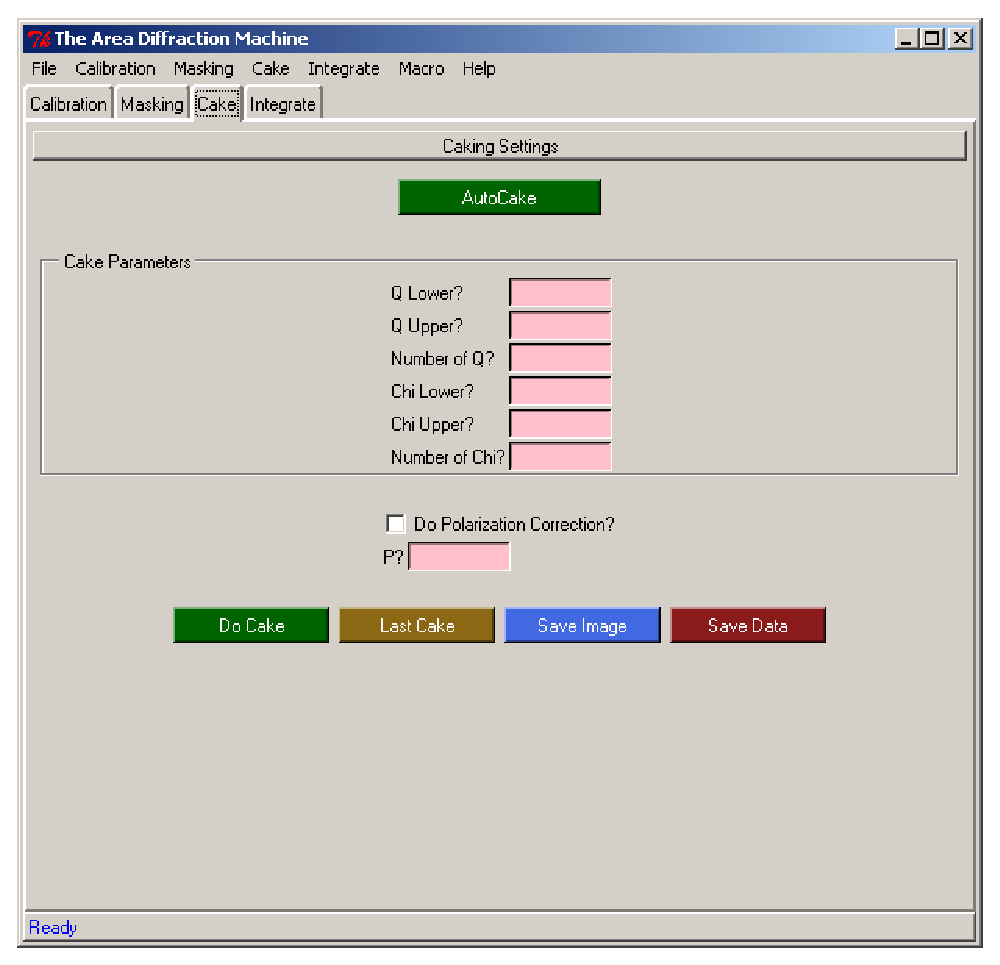
\includegraphics[scale=.75]{figures/caking_tab.eps}
    \caption{The caking tab of the program. This is
    where caking is done.} 
    \label{caking_tab}
\end{SCfigure}

Figure~\ref{caking_tab}
shows the \gui{Caking} tab. This is where caking is done. 
The program can only cake data after one or more diffraction 
files has been loaded into the program and after calibration
values for the particular diffraction image are loaded.
In order to cake, this program needs to know a range
in $Q$ and $\chi$ space that should be caked. 
This can be inputted with the \gui{Q Lower?}, \gui{Q Upper?}
\gui{Chi Lower?}, and \gui{Chi Upper?} inputs.
The program will also need to know how many $Q$ and $\chi$ bins to 
create when caking data. This can be inputted
with the \gui{Number of Q?} and \gui{Number of Chi?} inputs.
Once this is done, the \gui{Do Cake} button will cake the data. 

\begin{SCfigure}[1][htbp]
    \centering
    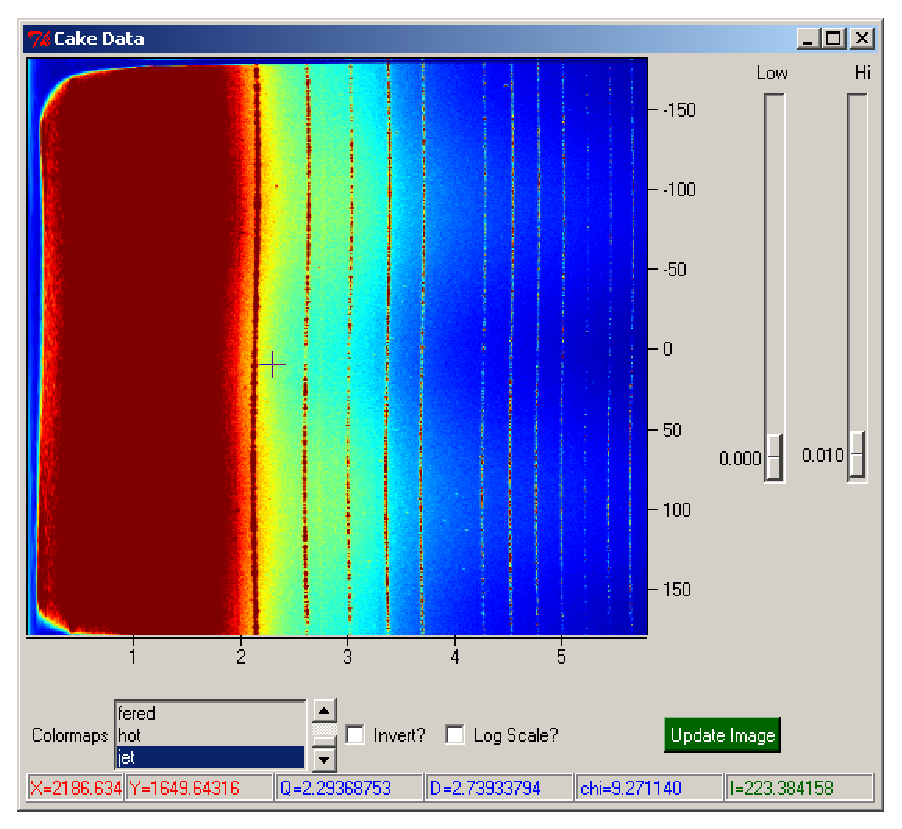
\includegraphics[scale=.75]{figures/cake_data_window.eps}
    \caption{The cake data window for
    the program. This window will open up after the
    data is caked. This window behaves exactly like 
    the diffraction data window.} 
    \label{cake_data_window}
\end{SCfigure}

After the cake finishes, the program will open a cake data
window which displays the cake data interactively.
The cake data window acts just like the diffraction
data window so everything in Chapter~\ref{viewing_data} 
carries over. The only real difference is that whenever
the caked data is zoomed into, the program will take
the selected zoom range and put it into the inputs on
the cake tab and the recake the image. The caked data can 
be taken to the previous zoom level
either by right clicking on the caked plot or by
pushing the \gui{Last Cake} button 

\section{AutoCake}

The program has a convenience button \gui{AutoCake}.
\gui{AutoCake} will guess a good range of $Q$ and $\chi$ 
values, put them into the input, and then push the 
\gui{Do Cake} button automatically. This will create a 
cake without much work. The program will pick a range
that puts every pixel from the 
diffraction image into the cake. It will pick
a bins sizes so that each pixel of the displayed 
cake data will correspond to one bin. This will ensure
that the cake looks as sharp as the computer can draw it.
After the display is resized, the number of bins will
change correspondingly. The next time \gui{AutoCake} is 
pushed, the cake window will again look sharp.

\section{\texorpdfstring{Displaying $Q$ and $\Delta Q$ Lines}
    {Displaying Q and delta Q Lines}}
    \label{cakeQlinesandpeaks}

If a $Q$ list has been loaded into the program, 
constant $Q$ lines or $\Delta Q$ lines can be 
displayed on top of the cake data. Remember that 
constant $Q$ lines on the diffraction image are straight
vertical lines on the caked plot. 
The program will display constant $Q$ lines or 
$\Delta Q$ lines on the caked plot whenever they 
should be displayed on the diffraction image. See 
section~\ref{displayconstQlines} and 
section~\ref{displayconstdQlines} for a discussion of 
displaying constant $Q$ lines on diffraction data.
Figure~\ref{constant_q_lines_on_cake_image} shows constant
$Q$ lines displayed on a caked plot and 
figure~\ref{constant_dq_lines_on_cake_image} shows constant
$\Delta Q$ lines displayed on a caked plot.

\begin{SCfigure}[1][htbp]
    \centering
    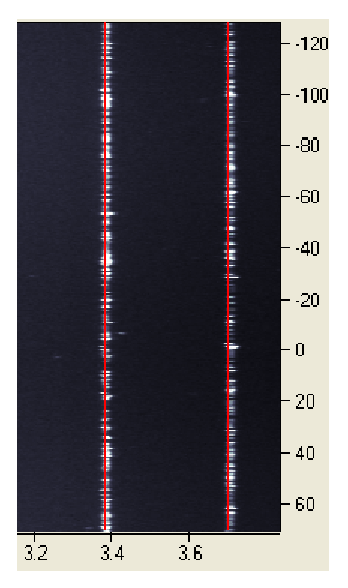
\includegraphics[scale=.75]{figures/constant_q_lines_on_cake_image.eps}
    \caption{The caked data window with constant $Q$ 
    lines drawn on top of it.}
    \label{constant_q_lines_on_cake_image}
\end{SCfigure}

\begin{SCfigure}[1][htbp]
    \centering
    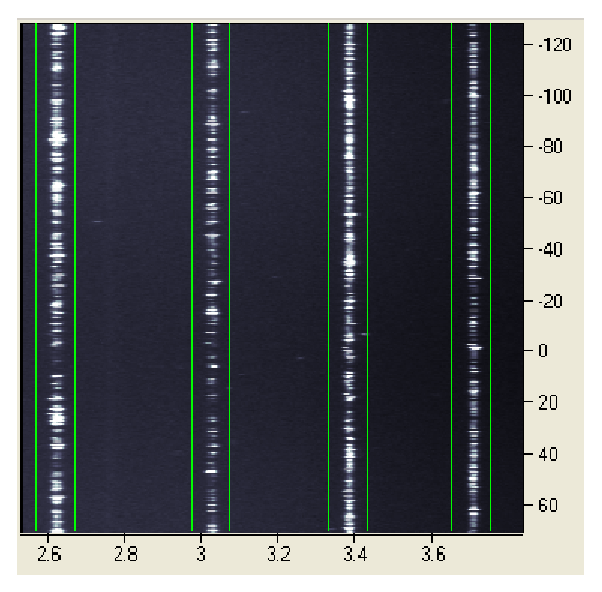
\includegraphics[scale=.75]{figures/constant_dq_lines_on_cake_image.eps}
    \caption{The caked data window with constant 
    $\Delta Q$ lines drawn on top of it.}
    \label{constant_dq_lines_on_cake_image}
\end{SCfigure}


\section{Displaying Peaks}\label{displaying_peaks_cake}

\begin{SCfigure}[1][htbp]
    \centering
    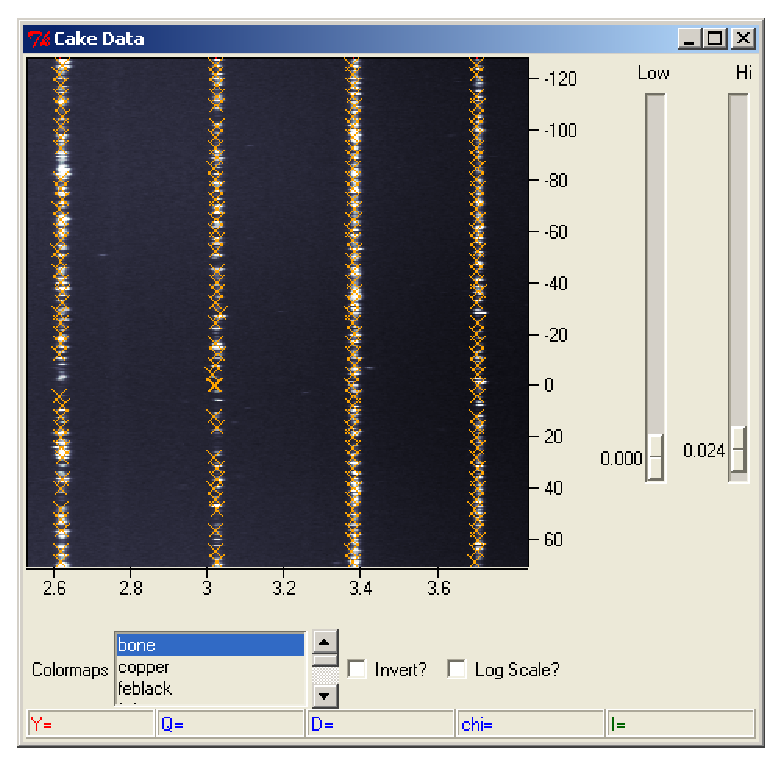
\includegraphics[scale=.75]{figures/peaks_on_cake_image.eps}
    \caption{The caked data window with diffraction 
    peaks drawn on top of it.}
    \label{peaks_on_cake_image}
\end{SCfigure}

Any peaks that the program finds when performing
a calibration can be displayed on top of the caked
data. The peaks will be displayed as crosses.
Figure~\ref{peaks_on_cake_image} shows peaks
displayed on a caked plot. Peaks will be displayed on 
the caked plot whenever they should be displayed on 
the diffraction image. See 
section~\ref{displaying_peaks_diffraction} for a
discussion of displaying peaks on diffraction data.
Being able to display $Q$ lines and peaks can
be very useful for checking if a calibration was 
done properly. Figure~\ref{calibration_cake} illustrates
this principle.

\begin{figure}[htb]
    \centering
    \subfloat[A bad calibration]{
    \label{bad_calibration_cake_zoom_peaks}
    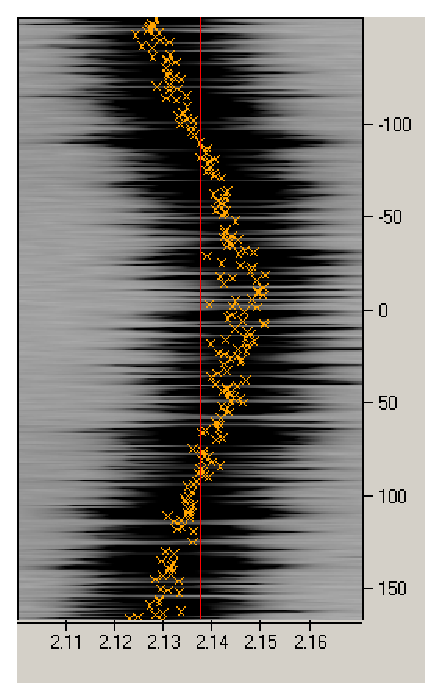
\includegraphics[scale=.75]{figures/bad_calibration_cake_zoom_peaks.eps}}\;\;
    \subfloat[A good calibration]{
    \label{good_calibration_cake_zoom_peaks}
    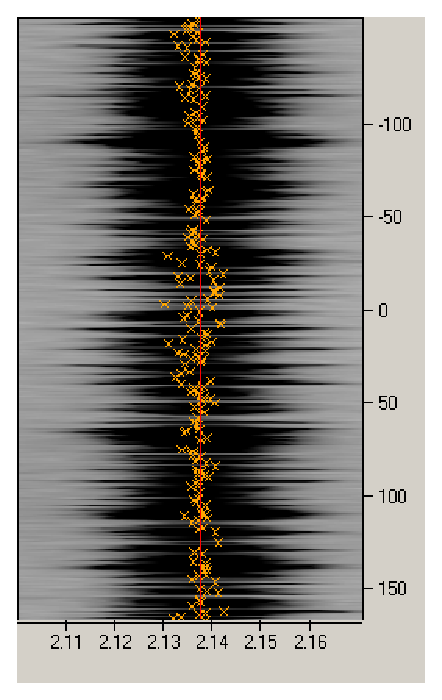
\includegraphics[scale=.75]{figures/good_calibration_cake_zoom_peaks.eps}}		
    \caption{displaying peaks and constant $Q$ lines on top of the 
    caked data can be used to tell if the data is properly calibrated. 
    If the calibration is good, all the peaks will cluster very close to
    a particular value of $Q$ line and 
    there will be no systematic variation of the diffraction peak. If 
    the calibration is bad, the diffraction peaks will have a systematic 
    distortion around some value of $Q$. This can be used to see if 
    the program is properly calibrating the data.}
    \label{calibration_cake}
\end{figure}


\section{Polarization Correction}
The program can apply a polarization correction to the
cake. The \gui{Do Polarization Correction?} check box
can be used to apply a polarization and the 
polarization value can be set with the \gui{P?} input.

\section{\texorpdfstring{Working in $2\theta$}{Working in 2theta}}

Caked plots can have $2\theta$ instead of $Q$ as one
of the axis.  This can be done by changing the program
to $2\theta$ mode by doing into the file menu and selecting 
the \gui{Work in 2theta} option. When this is selected,
all the names in the program will change from $Q$ to $2\theta$. 
For example, the program will have \gui{$2\theta$ Lower
}, \gui{$2\theta$ Upper}, \gui{Number of $2\theta$}. 
The program will display the cake image with
$2\theta$ as its axis. The \gui{Work in Q} option in the
file menu can be used to return the program to caking with$Q$
as one of the axis. This feature was introduces in version 2.0.0 
of the program.


\section{Saving Cake Images}

You can save caked data out as one of many popular image formats.
The program can save caked images as \gui{jpg}, \gui{gif}, \gui{eps}, 
\gui{pdf}, \gui{bmp}, \gui{png}, or \gui{tiff}.  When caked data is 
saved as an image, it will be saved out with whatever threshold masks,
polygon masks, $Q$ lines, $\Delta Q$ lines, and peaks were displayed 
over the caked data in the program.

\section{Saving Cake Data}

Caked data can also be saved as a plain text data file.
This can be done by pushing the \gui{Save Data} button and
selecting a destination. The format for caked files is just
a long comment string followed by the data as rows of numbers.
Here is an example:
\begin{lstlisting}[caption={'caked\_data.dat'}]
# Cake of: N:/data/LaB6_14_02_56.mar3450 
# Data Caked on Wed Mar 12 21:30:55 2008
# Calibration data used to make the cake:
#   x center:    1725.0000000 pixels
#   y center:    1725.0000000 pixels
#   distance:     125.2960000 mm
#   energy:     12735.3957721 eV
#   alpha:          0.0000000 degrees
#   beta:           0.0000000 degrees
#   rotation:       0.0000000 degrees
#   pixel length:     100.0000000 microns
#   pixel height:     100.0000000 microns
# A Polarization correction was applied
#   P = 0.500000
# A greater than mask was applied
#   Greater than mask = 1000.000000
# A Less Than Mask was applied
#   Less than mask = 10.000000
# Polygon mask(s) were applied
# Polygon(s) used in the analysis:
#   2400.10912343	1073.5706619
#   962.511627907	2282.88014311
#   2850.51520572	2572.86762075
#
#   1573.33631485	1215.47942755
#   1820.13416816	2893.70483005
#   2906.04472272	1573.33631485
# Cake range:
#   Q Lower = 0.000000
#   Q Upper = 6.726544
#   Number of Q = 560.000000
#   Q Step = 0.012012
#   chi Lower = -180.000000
#   chi Upper = 180.000000
#   Number of Chi = 560.000000
#   chi Step = 0.642857
# Note: pixels outside the diffraction image are saved as -1
#   Pixels greater than the greater than mask are saved as -2
#   Pixels less than the less than mask are saved as -3
#   Pixels inside of a polygon masks are saved as -4
# chi increased down. Q increases to the right
\end{lstlisting}
the comment string describes what state the program was in when the 
cake was done. It first lists the name of the diffraction 
file(s) that were caked. Next it lists the calibration parameters 
used when caking the data. Then is the polarization correction, the greater 
than mask and the less than mask that were used. It has the pixel 
coordinates of any polygons that were used when caking.  It then lists 
the range of the cake and the number of bins that were used.
The program sets the value of certain bins in the data
to special values. Bins that are outside of the diffraction
image are saved as -1. Bins that were masked because they were too 
large are saved as -2. Bins that were masked because they were too 
small are saved as -3. Bins that were inside a pixel mask are saved 
as -4. This is written in the comment string. 

The program tries to be smart about the comment string. If no 
masks were used, the comment string instead contains lines like
\begin{lstlisting}[caption={'Alternate Header'}]
# No greater than mask was applied
# No less than mask was applied
# No polygon masks were applied
\end{lstlisting}
If the program is working in $2\theta$ mode, the comment string will 
instead say something like
\begin{lstlisting}[caption={'Another Alternate Header'}]
#   2theta Lower = 0.000000
#   2theta Upper = 62.814525
#   number of 2theta = 560.000000
#   2theta Step = 0.112169
\end{lstlisting}


Then comes the data. As the header describes, each line in the
file is of constant $\chi$ and contains many numbers separated by
spaces. Each column is of constant $Q$. $\chi$ increases down and 
$Q$ increases to the right. The top left bin corresponds to
$Q$ lower and $\chi$ upper.
